\documentclass[border= 5mm]{standalone}
\usepackage{pgfplots}
\usepackage{tikz}   
\usepackage{animate}
\usepackage{adjustbox}
\usetikzlibrary{
	shapes,
	positioning,
	arrows,
	fit,
	backgrounds,
	calc,
	tikzmark,
	arrows.meta,
	shadows,
	automata}
\usepackage{pgfplots}
\pgfplotsset{compat=1.13} 
\usepackage{pgfplotstable}
   \definecolor{webgreen}{rgb}{0,.5,0}
\definecolor{webblue}{rgb}{0,0,.8}
\definecolor{webred}{rgb}{0.8, 0, 0}   
\definecolor{webbrown}{rgb}{.6,0,0}
\definecolor{webyellow}{rgb}{0.98,0.92,0.73}
\definecolor{webgray}{rgb}{.753,.753,.753}


\pgfplotscreateplotcyclelist{my color list}{%
	solid, color=webblue, every mark/.append style={solid, fill=webblue}, mark=*\\%
	densely dashdotted, color=webgreen, every mark/.append style={solid, fill=webred},mark=diamond*\\%
	densely dotted, color=webbrown, every mark/.append style={solid, fill=webgreen}, mark=triangle*\\%
	loosely dashed, color=webred, every mark/.append style={solid, fill=webbrown},mark=*\\%
	dotted, color=webblue, every mark/.append style={solid, fill=webyellow}, mark=square*\\%
	densely dotted, color=webgreen, every mark/.append style={solid, fill=gray}, mark=otimes*\\%
	dashed, color=webbrown, every mark/.append style={solid, fill=gray},mark=diamond*\\%
	densely dashed, every mark/.append style={solid, fill=gray},mark=square*\\%
	dashdotted, every mark/.append style={solid, fill=gray},mark=otimes*\\%
	dashdotdotted, every mark/.append style={solid},mark=star\\%
}


\begin{document}
	
	
	\begin{tabular}{cc}
	\maxsizebox{.5\textwidth}{!}
	{
		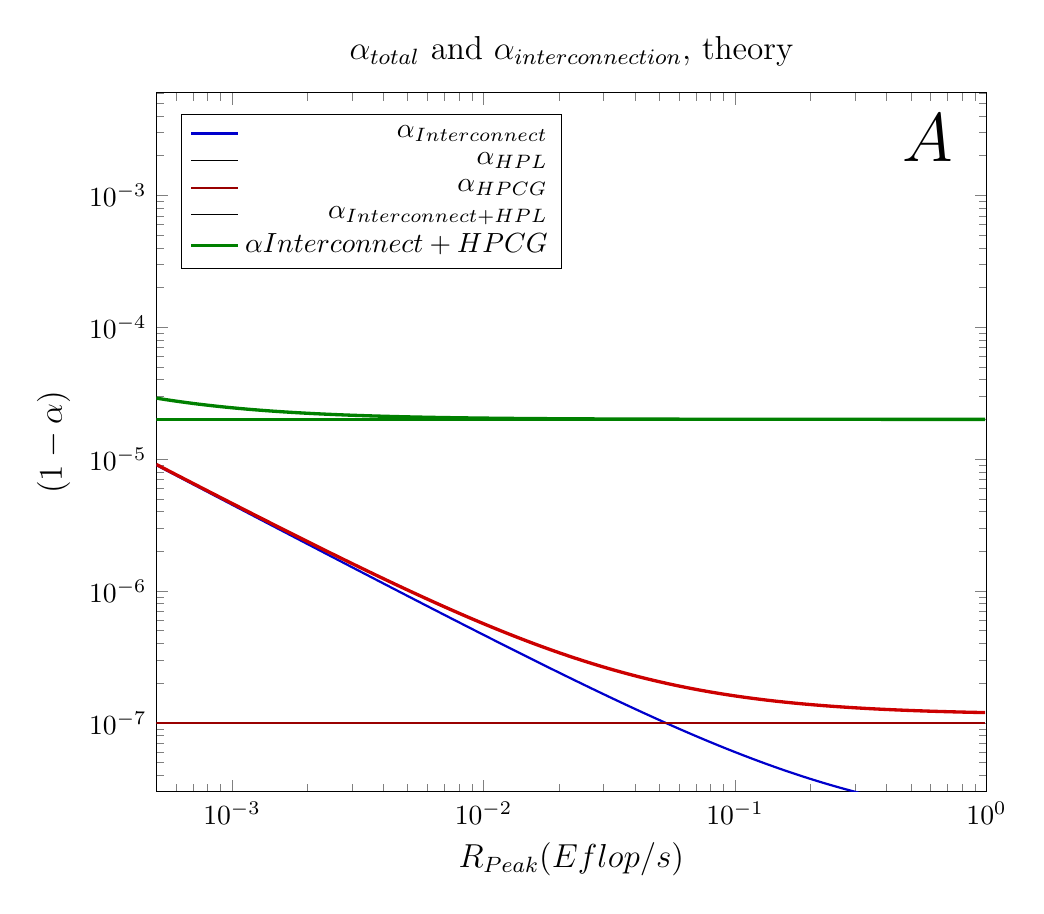
\begin{tikzpicture}%[scale=1.3]
		
		\def\constProcFreq{1}	% processor frequency, GHz
		\def\constMPE{1} % If MPE trick (see Taihulight) in use
		\def\constProcPerformance{(100*\constMPE)}  %processor performance, GFlops
		\def\constNoOfProcessors{x*1e9/\constProcPerformance} % x in Eflop/s
		\def\constTotalClocks{2e13} % Total measurement time, in ticks
		\def\constContextChange{1e4} % Time of context change, in ticks
		
		
		%% Derived 
		
		%\def\constProcFreq{1}	% processor frequency, GHz
		\def\constMicroSecToTicks{1e3*\constProcFreq}  % usec time to clock ticks
		%\def\constNoOfProcessors{x*1e8/64}
		% Calculate different \alpha contributions
		\def\constAlphaContext{\constContextChange/\constTotalClocks}
		\def\constAlphaLoop{\constNoOfProcessors/100/\constTotalClocks}
		\def\constAlphaOS{\constAlphaContext
			+\constAlphaLoop
		}
		\def\constAlphaNet{(1.5e-8*(1+.3/x))}
		% The sum of all contributions
		\def\constAlphaTotal{(\constAlphaSW%+\constAlphaOS
			+\constAlphaNet)}
		\def\constAlphaTotalHPCG{(\constAlphaSWHPCG%+\constAlphaOS
			+\constAlphaNet)}
		\def\constMinusAlpha{1-\constAlphaTotal}
		\def\constEfficiency{(\constNoOfProcessors*\constAlphaTotal+\constMinusAlpha)}
		\def\constRMax{x/2/\constEfficiency}
		\def\constPropagationDelay{\constNoOfProcessors*1e-6/2e-8*2e9/\constTotalClocks*1000}
		\def\constAlphaSW{1e-7}
		\def\constAlphaSWHPCG{2e-5}
		
		\pgfplotsset{
			%    scale only axis,
			%    scaled x ticks=base 10:3,
			xmin=0.001, xmax=1.1,
		}
		
		\begin{axis}[
		title={\large $\alpha_{total}$ and $\alpha_{interconnection}$,  theory},
		legend style={
			cells={anchor=east},
			legend pos={north west},
		},
		width=\textwidth,
		xlabel={\large $R_{Peak}(Eflop/s)$},
		ylabel={\large $(1-\alpha)$},
		xmin=5e-4, xmax=1,% x scale
		ymin=3e-8, ymax=6e-3, % y scale
		xmode=log,
		log basis x=10,
		ymode=log,
		log basis y=10,
		]
		% Handle the interconnect part
		\addplot[samples=501,domain=.0005:1,webblue,thick]
		{\constAlphaNet};\label{plot_net}
		\addlegendimage{/pgfplots/refstyle=plot_net}
		\addlegendentry{$\alpha_{Interconnect}$}
		
		% Handle the HPL part, constant SW
		\addplot[samples=501,domain=.0005:1,webbrown,thick]
		{\constAlphaSW }; \label{plot_HPL}
		\addlegendimage{/pgfplots/refstyle=plot_HPL}
		\addlegendentry{$\alpha_{HPL}$}
		
		% Handle the HPCG part, constant SW
		\addplot[samples=501,domain=.0005:1,webgreen,thick]
		{\constAlphaSWHPCG }; \label{plot_HPCG}
		\addlegendimage{/pgfplots/refstyle=plot_HPCG}
		\addlegendentry{$\alpha_{HPCG}$}
		
		%	Now the two sum HPL + interconnnectwith
		\addplot[samples=501,domain=.0005:1,webred,very thick]
		{\constAlphaTotal} ;\label{plot_total}
		\addlegendimage{/pgfplots/refstyle=plot_total}
		\addlegendentry{$\alpha_{Interconnect+HPL}$}
		
		\addplot[samples=501,domain=.0005:1,webgreen,very thick]
		{\constAlphaTotalHPCG} ;\label{plot_totalHPCG}
		\addlegendimage{/pgfplots/refstyle=plot_totalHPCG}
		\addlegendentry{$\alpha{Interconnect+HPCG}$}
		
		
		\end{axis}
		\draw node at (9.8, 8.3)  (A) {\Huge $A$};
		
		\end{tikzpicture}
	}	
	&
		\maxsizebox{.5\textwidth}{!}
		{
			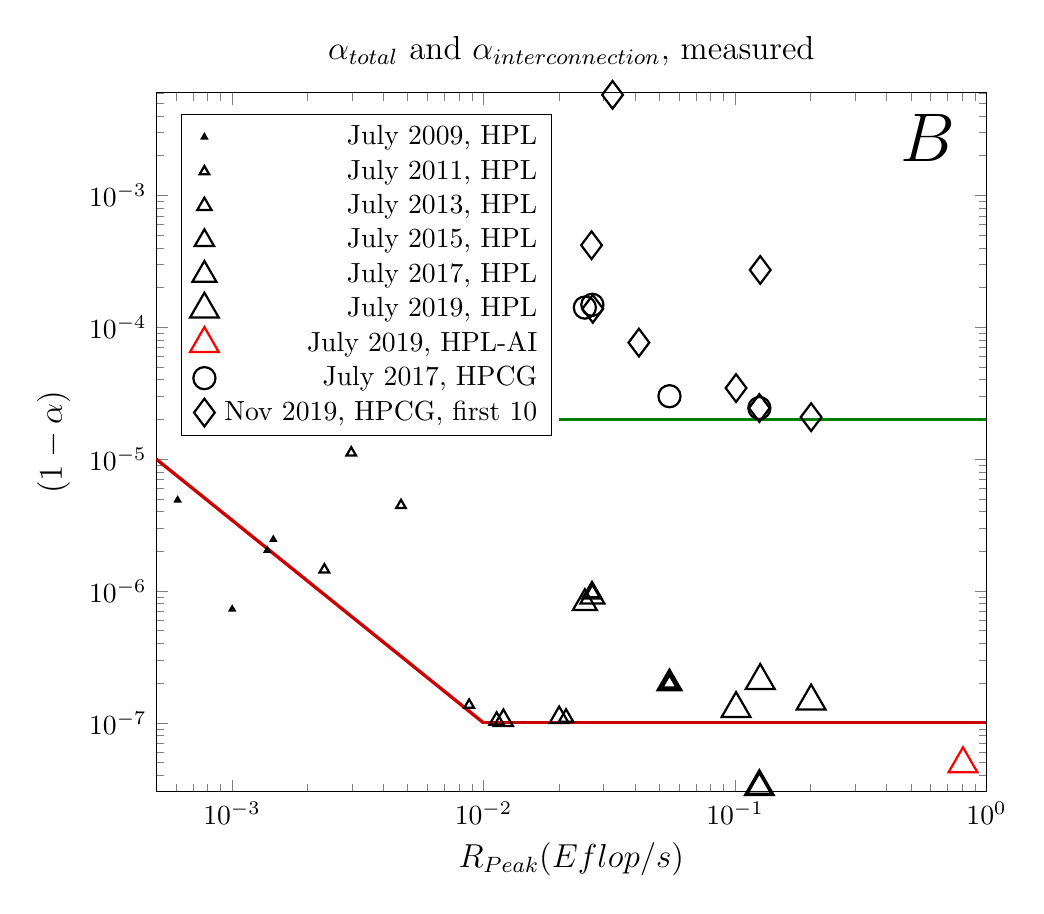
\begin{tikzpicture}%[scale=.55]
			\begin{axis}
			[
			title={\large $\alpha_{total}$ and $\alpha_{interconnection}$,  measured},
			width=\textwidth,
			%			cycle list name={my color list},
			legend style={
				cells={anchor=east},
				legend pos={north west},
			},
			xmin=5e-4, xmax=1,% x scale
			ymin=3e-8, ymax=6e-3, % y scale
			xlabel={\large $R_{Peak}(Eflop/s)$},
			/pgf/number format/1000 sep={},
			ylabel={\large $(1-\alpha)$},
			xmode=log,
			log basis x=10,
			ymode=log,
			log basis y=10,
			]
			
			% alpha, 2009 July, HPL
			\addplot[only marks,  mark=triangle,  mark size=1, thick] plot coordinates {
				(0.00146,2.456e-6)
				(0.001381,2.028e-6)
				(0.001002,7.27e-7)
				(0.000608,4.886e-6)
			};
			\addlegendentry{July 2009, HPL}
			
			alpha, 2011 July, HPL
			\addplot[only marks,  mark=triangle,  mark size=2, thick] plot coordinates {
				(0.00877,1.367e-7)
				(0.00470,4.464e-6)
				(0.00233,1.451e-6)
				(0.00298,1.117e-5)
			};
			\addlegendentry{July 2011, HPL}
			
			
			\draw[very thick,webred] (5e-4,10e-6) -- (1e-2,1.e-7);
				% alpha, 2013 July, HPL
				\addplot[only marks,  mark=triangle,  mark size=3, thick] plot coordinates {
					(0.0549,1.99e-7)
					(0.02711,9.65e-7)
					(0.0213,1.096e-7)
					(0.01128,1.04e-7)
				};
				\addlegendentry{July 2013, HPL}
				
				% alpha, 2015 July, HPL
				\addplot[only marks,  mark=triangle,  mark size=4, thick] plot coordinates {
					(0.0549,1.99e-7)
					(0.027,9.65e-7)
					(0.02,1.096e-7)
					(0.012,1.04e-7)
				};
				\addlegendentry{July 2015, HPL}
				
				% alpha, 2017 July, HPL
				\addplot[only marks,  mark=triangle,  mark size=5, thick] plot coordinates {
					(0.125,3.27e-8)
					(0.0549,1.99e-7)
					(0.0253,8.09e-7)
					(0.0271,9.06e-7)
				};
				\addlegendentry{July 2017, HPL}
				
				\addplot[only marks,  mark=triangle,  mark size=6, thick] plot coordinates {		
					(0.2008,1.46e-7)
					(0.126,2.09e-7)
					(0.125,3.27e-8)
					(0.101,1.28e-7)
				};
				\addlegendentry{July 2019, HPL}
				
				\addplot[only marks,  mark=triangle,  mark size=6, color=red, thick] plot coordinates {		
					(0.8064,0.488e-7)
				};
				\addlegendentry{July 2019, HPL-AI}
				\draw[very thick,webred] (1e-2,1e-7) -- (1e0,1.e-7);
					%\pause
					% alpha, 2017 July, HPCG
					\addplot[only marks,  mark=o,  mark size=4, thick] plot coordinates {	
						(0.125,2.44e-5)
						(0.0549,3.0e-5)
						(0.0253,1.41e-4)
						(0.0271,1.48e-4)
					};
					\addlegendentry{July 2017, HPCG}
					%\pause
					% alpha, 2019 July, HPCG
					\addplot[only marks,  mark=diamond,  mark size=5, thick] plot coordinates {		
						(0.2008,2.08e-5)
						(0.126,2.72e-4)
						(0.125,2.44e-5)
						(0.101,3.46e-5)
						(0.0272,1.38e-4)
						(0.0415,7.65e-5)
						(0.0326,5.79e-3)
						(0.0269,4.19e-4)
					};
					\addlegendentry{Nov 2019, HPCG, first 10}
					%\pause
					
					\draw[very thick,webgreen] (2e-2,2e-5) -- (1e0,2e-5);
			\end{axis}
			\draw node at (9.8, 8.3)  (B) {\Huge $B$};
			\end{tikzpicture}
	}
\end{tabular}
	
\end{document}
